% latex article template

% cheat sheet(eng): http://www.pvv.ntnu.no/~walle/latex/dokumentasjon/latexsheet.pdf
% cheat sheet2(eng): http://www.pvv.ntnu.no/~walle/latex/dokumentasjon/LaTeX-cheat-sheet.pdf
% reference manual(eng): http://ctan.uib.no/info/latex2e-help-texinfo/latex2e.html

% The document class defines the type of document. Presentation, article, letter, etc. 
\documentclass[12pt, a4paper]{article}

% packages to be used. needed to use images and such things. 
\usepackage[pdfborder=0 0 0]{hyperref}
\usepackage[utf8]{inputenc}
\usepackage[english]{babel}
\usepackage{graphicx}
\PassOptionsToPackage{hyphens}{url}

% hides the section numbering. 
\setcounter{secnumdepth}{-1}

% Graphics/image lications and extensions. 
\DeclareGraphicsExtensions{.pdf, .png, .jpg, .jpeg}
\graphicspath{{./images/}}

% Title or header for the document. 
\title{
TIØ4116: Ex7
}
% Author
\author{
	Magnus L. Kirø \\
}
\date{\today}

\begin{document}
\maketitle
\pagenumbering{arabic}

\section{Task 1}
Kommentar: oppgaven er (veldig) dårlig formulert.

\paragraph{A}
Gjennomsnittsrenten i perioden er 4.8
Så man burde velge en avkastningsrente på mer enn det. Noe sånt som 5.5 eller
6. 

\paragraph{B}
Nåverdien av selskapet er: 46397282318.8968. Mens overskuddet er på 139. 

Det er forutsatt verdiene i tabellen. 

\section{Task 2}
\paragraph{A} See figure 1.
% image example. 
\begin{figure}[h]
    \centering
    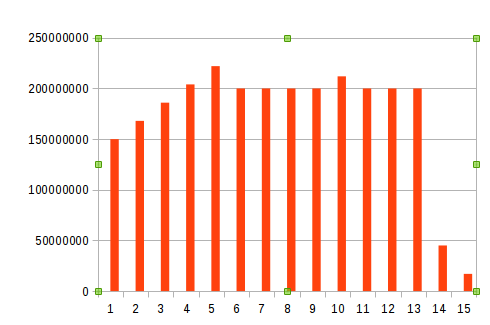
\includegraphics[width=\textwidth]{betstrom} 
    \label{fig:betstrom}
    \caption{}
Column A is the amount of money to be paid in each payment, while column B is
the year. Year: 1=2010, 5=2014, 9=2018, 13=2022.
\end{figure}

\paragraph{B}
Nåverdien av prosjektet er: 943809435.148704.  

\paragraph{C}
Mulighet 1 gir best avkastning over tid, gitt et innskudd i startfasen. 
Mulighet 3 gir best renteavkastning per år, men varer for kort til at det er
realistisk å skaffe finnansiering med en gang. 

Så en kombinasjon av mulighet 1 og 2 vil gi god avkastning over tid, og krever
middels innvesteringsvilje. 

Med innvestering på 410 mill i alternativ 1 og 2 vil man få gode resultater med
porteføljen. 

\section{Task 3}

\paragraph{A} Se figur 2.
\begin{figure}[h]
    \centering
    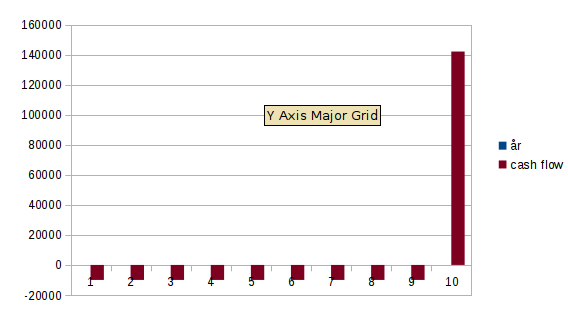
\includegraphics[width=\textwidth]{cashflow} 
    \label{fig:cashflow}
    \caption{}
The cashflow shows a yearly saving of 10000, and at the beginning of year 10 we
withdraw all the money. The initial r is 5\%. 
\end{figure}

\paragraph{B}
Verdien av obligasjonen er 1708 etter 9 år, med startverdi på 1200, og rente på
4\%.

\paragraph{C}
Den høyeste sansynligheten er å vinne 8 obligasjoner. Derfor er prisen 13664,
gitt obligasjonsverdien i B.

\paragraph{D}
0.8194.

\paragraph{E}
Given one payment the price has change with 267 for the final value to be a
about 900. 


\end{document}
